%%%%%%%%%%%%%%%%%%%%%%%%%%%%%%%%%%%%%%%%%
% Journal Article
% LaTeX Template
% Version 1.3 (9/9/13)
%
% This template has been downloaded from:
% http://www.LaTeXTemplates.com
%
% Original author:
% Frits Wenneker (http://www.howtotex.com)
%
% License:
% CC BY-NC-SA 3.0 (http://creativecommons.org/licenses/by-nc-sa/3.0/)
%
%%%%%%%%%%%%%%%%%%%%%%%%%%%%%%%%%%%%%%%%%

%----------------------------------------------------------------------------------------
%	PACKAGES AND OTHER DOCUMENT CONFIGURATIONS
%----------------------------------------------------------------------------------------

\documentclass[twoside]{article}

\usepackage{etex}

\usepackage{lipsum} % Package to generate dummy text throughout this template

\usepackage[sc]{mathpazo} % Use the Palatino font
\usepackage[T1]{fontenc} % Use 8-bit encoding that has 256 glyphs
\usepackage[utf8]{inputenc}
\linespread{1.05} % Line spacing - Palatino needs more space between lines
\usepackage{microtype} % Slightly tweak font spacing for aesthetics
\usepackage{amsmath}
\usepackage{listings}

\lstset{
  basicstyle=\small,
  breaklines=true
}

\usepackage[hmarginratio=1:1,top=32mm,columnsep=20pt]{geometry} % Document margins
\usepackage{multicol} % Used for the two-column layout of the document
\usepackage[hang, small,labelfont=bf,up,textfont=it,up]{caption} % Custom captions under/above floats in tables or figures
\usepackage{booktabs} % Horizontal rules in tables
\usepackage{float} % Required for tables and figures in the multi-column environment - they need to be placed in specific locations with the [H] (e.g. \begin{table}[H])
\usepackage{hyperref} % For hyperlinks in the PDF
\usepackage{multirow}

\usepackage{syntax}
\setlength{\grammarparsep}{5pt plus 1pt minus 1pt} % increase separation between rules
\setlength{\grammarindent}{6em} % increase separation between LHS/RHS 

\usepackage{lettrine} % The lettrine is the first enlarged letter at the beginning of the text
\usepackage{paralist} % Used for the compactitem environment which makes bullet points with less space between them

\usepackage{abstract} % Allows abstract customization
\renewcommand{\abstractnamefont}{\normalfont\bfseries} % Set the "Abstract" text to bold
\renewcommand{\abstracttextfont}{\normalfont\small\itshape} % Set the abstract itself to small italic text

\usepackage{tikz}
\usepackage{tikz-qtree}

\newcommand{\rparen}{)}

\usepackage{titlesec} % Allows customization of titles
\renewcommand\thesection{\Roman{section}} % Roman numerals for the sections
\renewcommand{\thesubsection}{\thesection\hspace{1mm}\alph{subsection}}
\titleformat{\section}[block]{\large\scshape\centering}{\thesection}{1em}{} % Change the look of the section titles
\titleformat{\subsection}[block]{\large}{\thesubsection\rparen}{1em}{} % Change the look of the section titles

\usepackage{fancyhdr} % Headers and footers
\pagestyle{fancy} % All pages have headers and footers
\fancyhead{} % Blank out the default header
\fancyfoot{} % Blank out the default footer
\fancyhead[C]{TDT4205 Compilers $\bullet$ Assignment One $\bullet$ \date{\today}} % Custom header text
\fancyfoot[RO,LE]{\thepage} % Custom footer text

%----------------------------------------------------------------------------------------
%	TITLE SECTION
%----------------------------------------------------------------------------------------

\title{\vspace{-15mm}\fontsize{24pt}{10pt}\selectfont\textbf{Theory for Assignment Three}} % Article title

\author{
    \large
    \textsc{Øyvind Robertsen} \\ % Your name
    \normalsize Norwegian University of Science \& Technology \\ % Your institution
    \normalsize \href{mailto:oyvinrob@stud.ntnu.no}{oyvinrob@stud.ntnu.no} % Your email address
    \vspace{-5mm}
}
\date{}

%----------------------------------------------------------------------------------------

\begin{document}

\maketitle % Insert title

\thispagestyle{fancy} % All pages have headers and footers

%----------------------------------------------------------------------------------------
%	ABSTRACT
%----------------------------------------------------------------------------------------

%\begin{abstract}

%\noindent \lipsum[1] % Dummy abstract text

%\end{abstract}

%----------------------------------------------------------------------------------------
%	ARTICLE CONTENTS
%----------------------------------------------------------------------------------------

\begin{multicols}{2} % Two-column layout throughout the main article text

    \section{Problem 1}
    \subsection{What is a symbol table, and why is it needed?}

    A symbol table is a data structure used in the semantic analysis phase of a compiler to maintain information regarding the identifiers in a program.
    Symbol tables solve many problems, the most prevalent of them being the need to maintain proper scoping (static or dynamic) and for a linker to able to resolve external references.
    In other words, a symbol table is used to know what an identifier means in the context of the program being compiled.

    \subsection{What kind of information is typically stored in a symbol table?}

    Symbol tables map identifiers to their types and location.
    Information regarding scope and the viability of an identifier within a scope is maintained via the presence (or lack thereof) of an identifier mapping in the symbol table.


    \section{Problem 2}
    \subsection{Describe the difference between static and dynamic typing.}

    A statically typed programming language requires the programmer to expicitly provide type information for all identifiers.
    In a dynamically typed language, the compiler/interpreter infers type information.

    \subsection{Describe the difference between strong and weak typing.}

    The terms strongly and weakly typed do not have a precise definition, but can be understood in terms of a strongly or weakly typed languages behaviour. 
    A strongly typed language is more likely to generate an error or refuse to compile a program that contains a mismatch between the type signature for a function parameter and the argument passed to the function.
    A weakly typed language on the other hand, will try to coerce the parameter to match the expected type via implicit type conversion and possibly produce unexpected results.
    In other words, wether a language is strongly or weakly typed describes how the compiler reacts to mismatching type signatures.

    \subsection{Explain why C is a static, weakly typed language.}

    All identifiers, both variables and functions, in C must be declared with a complete type signature.
    The type of an identifier will never be inferred at compile-/runtime.
    This makes C a statically typed language.

    Since no concise definition for weak and strong typing exists, it is hard to give a yes/no answer to wether or not a language is weakly/strongly typed or not.
    C is considered to be on the weaker end of the scale, due to it's tendency to perform implicit type conversions to make passed values match a type signature.

    \section{Problem 3}

    \subsection{Symbol table contents at line 16}

    With the symbol table organized as a stack of symbol tables, and each stack entry only showing the symbols added in the corresponding scope, we get the descending stack presented in table \ref{tab:prob3stack}.

    \begin{table*}[t]
        \centering
        \begin{tabular}{c|l}
            Stack entry & Contents \\ \hline
            1 & \{ \texttt{main} $\rightarrow$ VOID FUNC main()\} \\ \hline
            2 & \{ \texttt{a} $\rightarrow$ FLOAT := 1.0 \} \\ \hline
            3 & \{ \texttt{b} $\rightarrow$ BOOL := TRUE \} \\ \hline
            4 & \{ \texttt{a} $\rightarrow$ FLOAT := 2.0 \} \\ \hline
        \end{tabular}
        \caption{A (descending) stack showing the contents of the symbol table at line 16} \label{tab:prob3stack}
    \end{table*}

    \subsection{Result of printing}

    Line 16 will print the values $2.0$ and \texttt{TRUE}. The innermost scope assigns the value $2.0$ to the float \texttt{a} declared in the scope that is at the top of the stack at the time of execution. 
    The innermost scope also assigns \texttt{FALSE} to a boolean \texttt{b}, but the \texttt{b} in question is declared within that scope, so it does not effect the \texttt{b} declared in stack entry 3.

    \section{Problem 4}

    \subsection{Complete the SDD}

    The complete SDD is given in table \ref{tab:prob4sdd}. Assuming that a \texttt{current\_token}-function that returns the token currently being parsed exists.

    \begin{table*}[b]
        \centering
        \begin{tabular}{l|p{12cm}}
            Production & Semantic rule \\ \hline
            A $\rightarrow$ D = E & A.correct = (D.type == E.type) \\ \hline
            D $\rightarrow$ T \textbf{id} & D.type = T \\ \hline
            T $\rightarrow$ \textbf{int} | \textbf{float} & T = \texttt{current\_token} \\ \hline
            E $\rightarrow$ S B E &
\begin{lstlisting}
E.type = if B == + then
            if S.type == float or E.type == float then
                float
            else
                int
         else if S.type == E.type == float then
            float
         else if S.type == E.type == int then
            int
         else
            type_error
\end{lstlisting} \\ \hline
            E $\rightarrow$ U(E) & E.type = U.type \\ \hline
            E $\rightarrow$ S & E.type = S.type \\ \hline
            S $\rightarrow$ \textbf{int\_const} & S.type = \textbf{int} \\ \hline
            S $\rightarrow$ \textbf{float\_const} & S.type = \textbf{float} \\ \hline
            S $\rightarrow$ U(S) & S.type = U.type \\ \hline
            B $\rightarrow$ \textbf{+} | \textbf{/} & B = \texttt{current\_token} \\ \hline
            U $\rightarrow$ \textbf{tofloat} & U.type = float \\ \hline
            U $\rightarrow$ \textbf{toint} & U.type = int \\ \hline
        \end{tabular}
        \caption{The complete SDD for problem 4} \label{tab:prob4sdd}
    \end{table*}


    \subsection{Annotated parse trees}

    The annotated parse trees are given in figures \ref{fig:prob4bex1} and \ref{fig:prob4bex2}.

    \begin{figure*}[b]
        \centering
        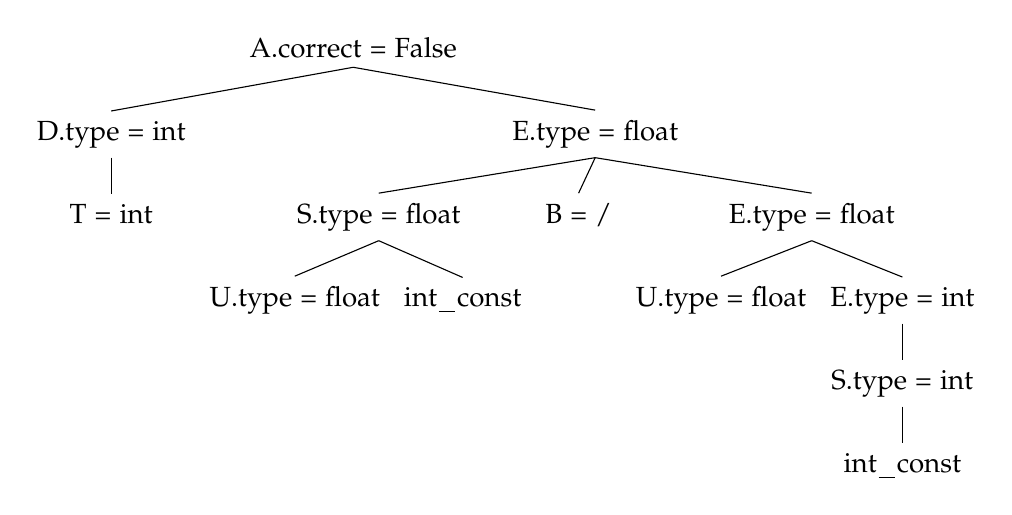
\begin{tikzpicture}[]
            \Tree [.{A.correct = False} 
                    [.{D.type = int} 
                        {T = int}
                    ]
                    [.{E.type = float} 
                        [.{S.type = float}
                            {U.type = float}
                            {int\_const}
                        ]
                        {B = /}
                        [.{E.type = float}
                            {U.type = float}
                            [.{E.type = int}
                                [.{S.type = int}
                                    {int\_const}
                                ]
                            ]
                        ]
                    ]
                ]
        \end{tikzpicture}
        \caption{Annotated parse tree for example 1, problem 4b} \label{fig:prob4bex2}
    \end{figure*}

    \begin{figure*}[b]
        \centering
        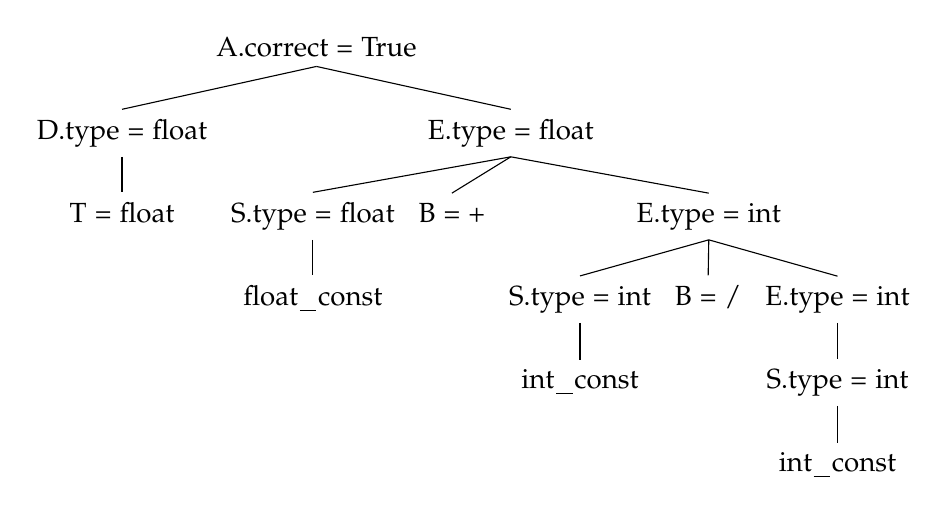
\begin{tikzpicture}[]
            \Tree [.{A.correct = True} 
                    [.{D.type = float} 
                        {T = float}
                    ]
                    [.{E.type = float} 
                        [.{S.type = float}
                            {float\_const}
                        ]
                        {B = +}
                        [.{E.type = int}
                            [.{S.type = int}
                                {int\_const}
                            ]
                            {B = /}
                            [.{E.type = int}
                                [.{S.type = int}
                                    {int\_const}
                                ]
                            ]
                        ]
                    ]
                ]
        \end{tikzpicture}
        \caption{Annotated parse tree for example 2, problem 4b} \label{fig:prob4bex1}
    \end{figure*}


\end{multicols}

\end{document}
